\begin{figure}[h]
  \centering
  \TODO{Embed figure inline.}

  \tikzstyle{vertex}=[]
  \tikzstyle{arrow}=[thick, -latex]

  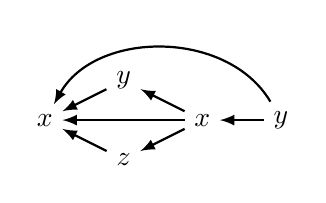
\begin{tikzpicture}
    \node[vertex] (x1) at (0, 0) {$x$};
    \node[vertex] (y1) at (1, 0.5) {$y$};
    \node[vertex] (y2) at (1, -0.5) {$z$};
    \node[vertex] (x2) at (2, 0) {$x$};
    \node[vertex] (z) at (3, 0) {$y$};

    \draw[arrow] (y1) to (x1);
    \draw[arrow] (y2) to (x1);
    \draw[arrow] (x2) to (y1);
    \draw[arrow] (x2) to (y2);
    \draw[arrow] (x2) to (x1);
    \draw[arrow, bend right=60] (z) to (x1);
    \draw[arrow] (z) to (x2);
  \end{tikzpicture}
  \caption{A conflict graph}\figlabel{ExampleConflictGraph}
\end{figure}
